% Created 2021-04-21 Wed 17:26
% Intended LaTeX compiler: pdflatex
\documentclass[11pt]{article}
\usepackage[utf8]{inputenc}
\usepackage[T1]{fontenc}
\usepackage{graphicx}
\usepackage{grffile}
\usepackage{longtable}
\usepackage{wrapfig}
\usepackage{rotating}
\usepackage[normalem]{ulem}
\usepackage{amsmath}
\usepackage{textcomp}
\usepackage{amssymb}
\usepackage{capt-of}
\usepackage{hyperref}
\usepackage[top=1in, bottom=1.25in, left=1.25in, right=1.25in]{geometry}
\usepackage{amsmath}
\setlength{\parindent}{0pt}

\usepackage[main,include]{embedall}
\IfFileExists{./\jobname.org}{\embedfile[desc=The original file]{\jobname.org}}{}





\usepackage{fvextra}
\fvset{
  commandchars=\\\{\},
  highlightcolor=white!95!black!80!blue,
  breaklines=true,
  breaksymbol=\color{white!60!black}\tiny\ensuremath{\hookrightarrow},
}
\renewcommand\theFancyVerbLine{\footnotesize\color{black!40!white}\arabic{FancyVerbLine}}

\usepackage[many]{tcolorbox}
\DeclareTColorBox[]{Code}{}%
{enhanced,
  colback=white!97!black,
  colframe=white!94!black, boxrule=0.5pt,
  fontupper=\color{EFD}\footnotesize,
  arc=2.5pt, outer arc=2.5pt,
  boxsep=2pt, left=2pt, right=2pt, top=1pt, bottom=0.5pt,
  breakable}

\definecolor{EFD}{HTML}{383a42}
\newcommand{\EFD}[1]{\textcolor{EFD}{#1}} % default
\definecolor{EFk}{HTML}{e45649}
\newcommand{\EFk}[1]{\textcolor{EFk}{#1}} % font-lock-keyword-face
\definecolor{EFd}{HTML}{84888b}
\newcommand{\EFd}[1]{\textcolor{EFd}{\textit{#1}}} % font-lock-doc-face
\definecolor{EFt}{HTML}{986801}
\newcommand{\EFt}[1]{\textcolor{EFt}{#1}} % font-lock-type-face
\definecolor{EFs}{HTML}{50a14f}
\newcommand{\EFs}[1]{\textcolor{EFs}{#1}} % font-lock-string-face
\definecolor{EFw}{HTML}{986801}
\newcommand{\EFw}[1]{\textcolor{EFw}{#1}} % font-lock-warning-face
\definecolor{EFb}{HTML}{a626a4}
\newcommand{\EFb}[1]{\textcolor{EFb}{#1}} % font-lock-builtin-face
\definecolor{EFct}{HTML}{9ca0a4}
\newcommand{\EFct}[1]{\textcolor{EFct}{#1}} % font-lock-comment-face
\definecolor{EFc}{HTML}{b751b6}
\newcommand{\EFc}[1]{\textcolor{EFc}{#1}} % font-lock-constant-face
\definecolor{EFpp}{HTML}{4078f2}
\newcommand{\EFpp}[1]{\textcolor{EFpp}{\textbf{#1}}} % font-lock-preprocessor-face
\definecolor{EFnc}{HTML}{4078f2}
\newcommand{\EFnc}[1]{\textcolor{EFnc}{\textbf{#1}}} % font-lock-negation-char-face
\definecolor{EFv}{HTML}{6a1868}
\newcommand{\EFv}[1]{\textcolor{EFv}{#1}} % font-lock-variable-name-face
\definecolor{EFf}{HTML}{a626a4}
\newcommand{\EFf}[1]{\textcolor{EFf}{#1}} % font-lock-function-name-face
\definecolor{EFcd}{HTML}{9ca0a4}
\newcommand{\EFcd}[1]{\textcolor{EFcd}{#1}} % font-lock-comment-delimiter-face
\definecolor{EFrc}{HTML}{4078f2}
\newcommand{\EFrc}[1]{\textcolor{EFrc}{\textbf{#1}}} % font-lock-regexp-grouping-construct
\definecolor{EFrb}{HTML}{4078f2}
\newcommand{\EFrb}[1]{\textcolor{EFrb}{\textbf{#1}}} % font-lock-regexp-grouping-backslash
\definecolor{EFhn}{HTML}{da8548}
\newcommand{\EFhn}[1]{\textcolor{EFhn}{\textbf{#1}}} % highlight-numbers-number
\definecolor{EFhq}{HTML}{4078f2}
\newcommand{\EFhq}[1]{\textcolor{EFhq}{#1}} % highlight-quoted-quote
\definecolor{EFhs}{HTML}{986801}
\newcommand{\EFhs}[1]{\textcolor{EFhs}{#1}} % highlight-quoted-symbol
\definecolor{EFrdi}{HTML}{4078f2}
\newcommand{\EFrdi}[1]{\textcolor{EFrdi}{#1}} % rainbow-delimiters-depth-1-face
\definecolor{EFrdii}{HTML}{a626a4}
\newcommand{\EFrdii}[1]{\textcolor{EFrdii}{#1}} % rainbow-delimiters-depth-2-face
\definecolor{EFrdiii}{HTML}{50a14f}
\newcommand{\EFrdiii}[1]{\textcolor{EFrdiii}{#1}} % rainbow-delimiters-depth-3-face
\definecolor{EFrdiv}{HTML}{da8548}
\newcommand{\EFrdiv}[1]{\textcolor{EFrdiv}{#1}} % rainbow-delimiters-depth-4-face
\definecolor{EFrdv}{HTML}{b751b6}
\newcommand{\EFrdv}[1]{\textcolor{EFrdv}{#1}} % rainbow-delimiters-depth-5-face
\definecolor{EFrdvi}{HTML}{986801}
\newcommand{\EFrdvi}[1]{\textcolor{EFrdvi}{#1}} % rainbow-delimiters-depth-6-face
\definecolor{EFrdvii}{HTML}{4db5bd}
\newcommand{\EFrdvii}[1]{\textcolor{EFrdvii}{#1}} % rainbow-delimiters-depth-7-face
\definecolor{EFrdiix}{HTML}{80a880}
\newcommand{\EFrdiix}[1]{\textcolor{EFrdiix}{#1}} % rainbow-delimiters-depth-8-face
\definecolor{EFrdix}{HTML}{887070}
\newcommand{\EFrdix}[1]{\textcolor{EFrdix}{#1}} % rainbow-delimiters-depth-9-face
\author{Jake Moss - s46409665}
\date{\today}
\title{Project}
\hypersetup{
 pdfauthor={Jake Moss - s46409665},
 pdftitle={Project},
 pdfkeywords={},
 pdfsubject={},
 pdfcreator={Emacs 28.0.50 (Org mode 9.5)}, 
 pdflang={English}}
\begin{document}

\maketitle
\tableofcontents



\section{Introduction}
\label{sec:org124c731}
\subsection{Project aims}
\label{sec:org0cbc82a}
The goal of this project was to provide a new and somewhat unique visualisations of chess games. I plan to do this by plotting various positions of events such as
\begin{itemize}
\item[{$\boxtimes$}] Captures
\item[{$\square$}] Checks
\item[{$\square$}] Checkmates
\end{itemize}
In addition to these I plan to show when these events happen throughout games.

The purpose of this project is to show the positional differences between different levels of play and over time. This is something not often visualised within the community thus I thought it would be a unique take on some common statistic.
\subsection{Obtaining data}
\label{sec:org4e20b33}
\subsubsection{Sources}
\label{sec:org57e0bc1}
Chess games are found freely on the internet from many archives such as \href{https://www.pgnmentor.com/files.html}{PGN Mentor}. From here I am able to download thousands of games at mass using a FireFox extension. However as most preserved games are of tournaments and high skill players this data doesn't not sure what happens in common games. To help mitigate this I can use the public API's from \href{https://lichess.org/}{Lichess} and \href{https://www.chess.com/}{Chess.com} to gather games from friends and players from various ELO's.

To pull games from Chess.com I use this bash command to gather the PGN files from individual months and write them to a single file as Chess.com does not support downloading of all games at once.
\begin{Code}
\begin{Verbatim}[]
\color[HTML]{383a42}\EFk{for} g\EFk{ in} \$\textcolor[HTML]{4078f2}{(}\textcolor[HTML]{986801}{\textit{curl}} -Ls https://api.chess.com/pub/player/\$\EFv{PLAYERNAME}/games/archives | jq -rc \EFs{".archives[]"}\textcolor[HTML]{4078f2}{)} ; \EFk{do} \textcolor[HTML]{986801}{\textit{curl}} -Ls \EFs{"}\textcolor[HTML]{b751b6}{\textbf{\$}}\textcolor[HTML]{6a1868}{g}\EFs{"} | jq -rc \EFs{".games[].pgn"} ; \EFk{done} >> games.pgn
\end{Verbatim}
\end{Code}

Lichess easily allows for downloading of an entire players archive at once with
a simple \texttt{curl}.
\begin{Code}
\begin{Verbatim}[]
\color[HTML]{383a42}\textcolor[HTML]{986801}{\textit{curl}} https://lichess.org/games/export/\$\EFv{PLAYERNAME} > games.pgn
\end{Verbatim}
\end{Code}
\subsubsection{PGN Format}
\label{sec:org756c669}
The most common format used to store chess games is \href{https://en.wikipedia.org/wiki/Portable\_Game\_Notation}{Portable Game Notation}. It is a human readable plain text notation which stores individual moves rather than the board states. While this is considerably more efficient for both storage and computation it makes extracting data that isn't explicitly given difficult and costly.

The \href{http://www.saremba.de/chessgml/standards/pgn/pgn-complete.htm}{standard} defines a required \href{http://www.saremba.de/chessgml/standards/pgn/pgn-complete.htm\#c8.1.1}{seven tag roster} and allows for optional tags such as \texttt{WhiteElo} and \texttt{BlackElo}. Each move is stored in \href{https://en.wikipedia.org/wiki/Algebraic\_notation\_(chess)}{Standard Algebraic Notation}, which describes the change in board state such as captures, checks, and promotions.

SAN comes in a varsity of formats short, long, or minimal. Each variant encodes moves with different levels of detail. Unfortunately no single variant is used in all PGN databases, although it is rare for the format to change from within a database.

A standard might look something like this
\begin{verbatim}
[Event "WCh 2018"]
[Site "London ENG"]
[Date "2018.11.09"]
[Round "1"]
[White "Caruana, Fabiano"]
[Black "Carlsen, Magnus"]
[Result "1/2-1/2"]
[WhiteTitle "GM"]
[BlackTitle "GM"]
[WhiteElo "2832"]
[BlackElo "2835"]
[ECO "B31"]
[Opening "Sicilian"]
[Variation "Nimzovich-Rossolimo attack (with ...g6, without ...d6)"]
[WhiteFideId "2020009"]
[BlackFideId "1503014"]
[EventDate "2018.11.09"]

1. e4 c5 2. Nf3 Nc6 3. Bb5 g6 ... 115. Ra8 1/2-1/2
\end{verbatim}
Tags preface the game in \texttt{[]}, often far more than required are provided. These tags are referred to as the headers. The moves themselves are listed in SAN with the result at the end.

Due to the variation within each format and the format implicitly encoding data I wished to extract I chose not to write my own PGN parser and invalidator and instead to use an existing popular library, \href{https://github.com/niklasf/python-chess}{python-chess}.

I would have preferred to use an alternative notation, \texttt{Reversible algebraic}, as it explicitly states the captured piece and its position within plain text. This would have allowed me to directly gather the data using regex without playing out each game.
\subsection{Motivation}
\label{sec:orgf700212}
As someone who does not play chess this is a strange choice of a project.
\section{Data Processing}
\label{sec:orgfb6978a}
\subsection{Tools used}
\label{sec:orgdb78b19}
In this project I make use of 4 libraries
\begin{itemize}
\item \href{https://github.com/niklasf/python-chess}{python-chess}
Used to handle the complex move validation and PGN parsing required to step though games.
\item \href{https://matplotlib.org/}{matplotlib}
Standard plotting library.
\item \href{https://seaborn.pydata.org/}{seaborn}
A high level plotting library built on \texttt{matplotlib}.
\item \href{https://numpy.org/}{numpy}
Standard scientific computing library. Within this project it is used to for its \texttt{pandas} optimisations, and reshape function.
\item \href{https://pandas.pydata.org/}{pandas}
Data frames provide an efficient way to store and conditionally select games based on metadata.
\end{itemize}
\subsection{Meta Data Extraction}
\label{sec:orgea88f54}
To extract the metadata from a game the PGN file is read using standard python methods and the game object is initialised using the \texttt{aggergate} function from the \texttt{aggergation.py} module. From the game object the headers are extracted into a dictionary and a data frame is created consisting of the headers are column titles and rows as individual games.

\begin{center}
\begin{tabular}{lllllllll}
 & SAN string & Black & White & Result & BlackElo & WhiteElo & Date & \ldots{}\\
\hline
1 & \texttt{SAN string} & \texttt{name} & \texttt{name} & \texttt{string} & \texttt{int} & \texttt{int} & \texttt{DateTime} & \ldots{}\\
\ldots{} &  &  &  &  &  &  &  & \\
\end{tabular}
\end{center}


\subsection{Extracting Implicit Data}
\label{sec:org8b58e87}
To extract the ``implicit data'' such as piece captures each game must be played out in its entirety with each move analysed.
\subsection{Data storage}
\label{sec:orgc31b0eb}
\section{Data Analysis}
\label{sec:org2a4fc91}
\subsection{Local and Global Normalisation}
\label{sec:orgc010276}
Within the heat map grid plots, each map shares the colour bar on the right. To accomplish this each square with each map is normalised to the sum of the local grid so that the map represents proportion instead of frequency. From this we now know that the maximum value is \texttt{1} and the colour bar can be calibrated to \texttt{[0,1]}. However, as the proportion of lost pieces rarely gets close to \texttt{0.5} let alone \texttt{1}, the colours become hard to differentiate.

To remedy this I set the maximum of all local maximums to the max of the colour bar. This made it so that each plot is proportional to itself and the colouring is consistent between plots.
\begin{center}
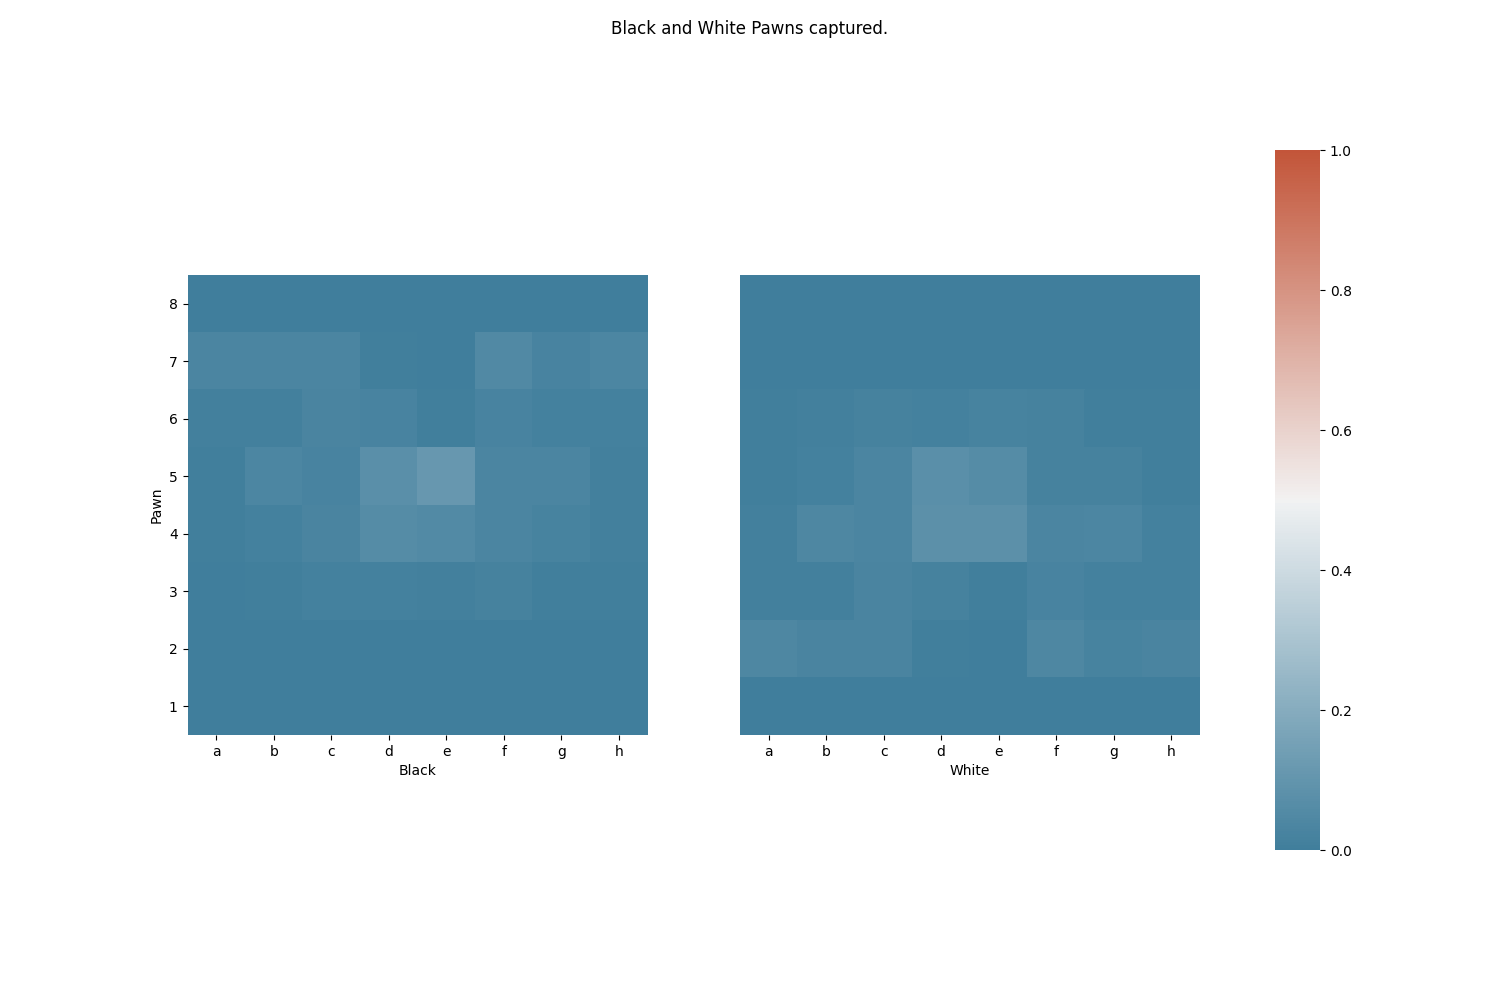
\includegraphics[width=300]{images/DaenaliaEvandruile_HEATMAP_Pawn_WHITE_EXAMPLE_1_WITH_WRONG_COLOUR.png}
\end{center}

\begin{center}
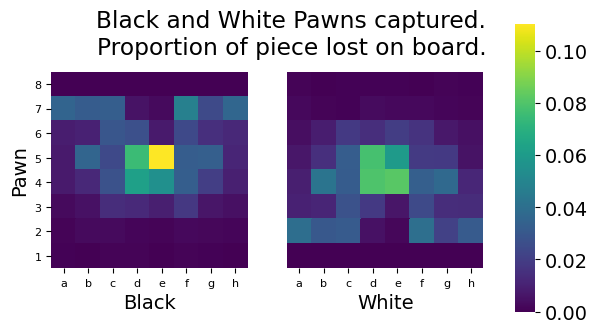
\includegraphics[width=300]{images/DaenaliaEvandruile_HEATMAP_Pawn.png}
\end{center}

A similar strategy was employed to ensure the histograms and kernel density plots shared the same axis.

\subsection{Difficulties and issues}
\label{sec:orgdf6e5f4}
\subsubsection{Pawn capture on 8th rank}
\label{sec:org8c1d1fd}
Some pawn capture heat maps show a capture on the 8th rank (furthest row away from the starting position). According to the FIDE
\begin{quote}
3.7e) When  a  pawn  reaches  the  rank  furthest  from  its  starting  position  it  must  be  exchanged  as  part  of  the  same  move  on  the  same  square  for  a  new queen,  rook,  bishop  or  knight  of  the  same  colour.  The  player’s  choice  is  not  restricted  to  pieces  that  have  been  captured  previously.  This  exchange  of  a  pawn  for  another  piece  is  called ‘promotion’ and the effect of the new piece is immediate.
\cite{FIDE}
\end{quote}
Thus a pawn can never be captured on the 8th rank.

This bug likely occurs due to how the detection of captures and handling of positions works. While promotions are accounted for there is a specific edge case that persists.

\begin{Code}
\begin{Verbatim}[]
\color[HTML]{383a42}\EFk{def} \EFf{piece\_delta}(board: chess.Board, count: \EFb{int}, piece\_count: Dict[\EFb{int}, \EFb{int}],
                colour: \EFb{bool}) -> \EFv{Tuple}[\EFb{int}, \EFb{int}, \EFb{int}]:
    piece\_position = (\EFhn{0}, \EFhn{0}, \EFhn{0})
    \EFk{for} key, value \EFk{in} piece\_count.items():
        \EFv{current\_count} = \EFb{bin}(board.pieces\_mask(key, colour)).count(\EFs{'1'})
        \EFk{if} current\_count < \EFv{value}: \EFcd{\# }\EFct{Detects lost based on previous state
 }           piece\_position = (key, uci\_to\_1d\_array\_index(board.peek().uci()), count)
            \EFv{piece\_count}[\EFv{key}] = current\_count \EFcd{\# }\EFct{Modify by object-reference
 }           \EFk{break}
        \EFk{elif} current\_count > \EFv{value}: \EFcd{\# }\EFct{Accounts for promotion
 }           piece\_count[\EFv{key}] = current\_count \EFcd{\# }\EFct{Modify by object-reference
 }           \EFv{piece\_count}[chess.\EFv{PAWN}] = \EFb{bin}(board.pieces\_mask(chess.PAWN, colour)).count(\EFs{'1'})  \EFcd{\# }\EFct{Account for pawn count change
 }           \EFk{break}
    \EFk{return} piece\_position \EFcd{\# }\EFct{piece id, position, count}
\end{Verbatim}
\end{Code}

This code block works by making mask of the current board state. This returns a boolean bitboard consisting only of the piece requested.
\begin{table}[htbp]
\caption{Piece mask of Black starting pawns}
\centering
\begin{tabular}{|rrrrrrrr|}
\hline
0 & 0 & 0 & 0 & 0 & 0 & 0 & 0\\
1 & 1 & 1 & 1 & 1 & 1 & 1 & 1\\
0 & 0 & 0 & 0 & 0 & 0 & 0 & 0\\
0 & 0 & 0 & 0 & 0 & 0 & 0 & 0\\
0 & 0 & 0 & 0 & 0 & 0 & 0 & 0\\
0 & 0 & 0 & 0 & 0 & 0 & 0 & 0\\
0 & 0 & 0 & 0 & 0 & 0 & 0 & 0\\
0 & 0 & 0 & 0 & 0 & 0 & 0 & 0\\
\hline
\end{tabular}
\end{table}
This is then counted and used as the number of current pieces of the piece type present. As this method only keeps track of the number of pieces on the board at once and relies on the previous state to detect a capture it can be easily broken by a change in the piece count other than a capture. For example promotions, as promotions exchange a pawn in favour of another piece type the piece change is not negative. Although this is accounted for there is still a specific edge case which is not caught.

After a pawn promotes, if it is immediately captured the lost piece is still attributed as a pawn. I was unable to squash this bug.
\subsubsection{Timezones and my ignorance of them}
\label{sec:org4ff4bab}
In 1918, Russia switched from the Julian calendar to the Gregorian calendar. In the switch the dates from   1st–13th of February. In doing so breaking any naive date comparison implementation from before the switch to after.

As Tom Scott put it \href{https://youtu.be/-5wpm-gesOY}{``What you learn after dealing with time zones, is that what you do is put away from code and you don't try and write anything to deal with this. You look at the people who have been there before you. You look at the first people, the people who have dealt with this before, the people who have built the spagetti code, and you thank them very much for making it open source.''}. Rather than dealing with time zones the \texttt{pd.to\_datetime()} method was employed to correctly handle dates. Although my use-case is not very complicated it is better to use code that I can trust.

\subsubsection{Storing game object in Data frame}
\label{sec:org02f7487}
I ran into a lot of issues storing a game object within the same data frame as the metadata. The object would be cast to its string representation due to pandas seeing the rest of the data frame as strings. This string representation would just be the original PGN game making it very inefficient to have to prase the game again.

To over come this I stored the game objects with a normal list and made sure to sync the index of the data frame to the corresponding game within the list. As data frame indexing starts at \texttt{0} there is not offset. For example, the row of index \texttt{7} of the data frame corresponds to game of index \texttt{8} within the game list.
\subsubsection{Kernel density plots report negative time}
\label{sec:orgdd8392d}
KDE plots apply smoothing to give a continuous and appealing look. Unfortunately this smooths bleeds over to the negative x-axis. This is wrong, move numbers cannot be negative, however, truncating the axis can produce jarring plots.
\begin{center}
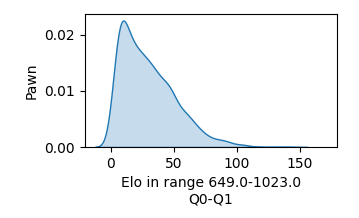
\includegraphics[height=0.2\textwidth]{images/KDE negative values.png}
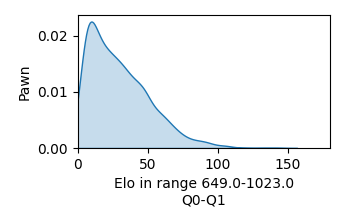
\includegraphics[height=0.2\textwidth]{images/KDE bad smoothing.png}
\end{center}

As the negative x-axis being incorrect and misleading I chose to truncate all histogram and KDE plots.
\section{Conclusion}
\label{sec:orga97ea47}
\subsection{Results}
\label{sec:orgf84b4f2}
\section{Reflection}
\label{sec:org5fc0047}
\section{References}
\label{sec:org9f5945b}
\bibliographystyle{plain}
\bibliography{project}
\end{document}
